\documentclass[10pt]{beamer}
\beamertemplatenavigationsymbolsempty
\usecolortheme{beaver}
% \usetheme{Madrid}
\usefonttheme{professionalfonts}
\usepackage[utf8]{inputenc}
\usepackage[T1]{fontenc}
\usepackage{amsmath, amssymb, amsthm}
% \usepackage[russian]{babel}
\usepackage[english]{babel}
\usepackage{hyperref}
\usepackage{algorithm, algorithmic}
\usepackage{graphicx}
\usepackage{booktabs}

\title{A Fine-Grained Analysis on Distribution Shift}
\author{
Authors: Olivia Wiles, Sven Gowal, Florian Stimberg,\\
Sylvestre-Alvise Rebuffi, Ira Ktena,\\
Krishnamurthy (Dj) Dvijotham, Taylan Cemgil\\[2mm]
\small Talk by Muhammadsharif Nabiev
}
\institute{Moscow Institute of Physics and Technology}
\date{2025}

\begin{document}

% ----------------------- Title -----------------------
\begin{frame}
  \titlepage
\end{frame}

% ------------- Motivation & central question ---------
\begin{frame}{Motivation \& central question}
\textbf{Robustness problem.}
\begin{itemize}
  \item Models are trained on one data distribution, but deployed on another (new hospitals, cameras, lighting, subgroups, \dots).
  \item Under such \emph{distribution shifts}, accuracy can drop sharply and unpredictably.
\end{itemize}

\medskip
\textbf{Gap.}
\begin{itemize}
  \item Many robustness / domain generalization methods exist.
  \item But we lack a \emph{unified, controlled} way to:
  \begin{itemize}
    \item define different types of shift;
    \item and compare methods across these shifts and datasets.
  \end{itemize}
\end{itemize}

\medskip
\textbf{Question.}
Can we define important distribution shifts in a principled way and
systematically evaluate existing methods under these shifts?
\end{frame}

% ------------------ Core framework -------------------
\begin{frame}{Core framework: attributes and shifts}
\textbf{Latent factorisation view.} 
\begin{itemize}
  \item Data described by discrete attributes
  \[
    y^1, y^2, \dots, y^K \in \mathcal{A}^k,
  \]
  e.g.\ label of interest $y^\ell$ (shape, tumor presence) + nuisance attributes $y^a$ (color, hospital, location).
  \item Assume a shared conditional generator
  \[
    p(\mathbf{x} \mid y^1,\dots,y^K)
  \]
  across train and test.
\end{itemize}

\medskip
\textbf{Distribution shift (in this paper).}
\begin{itemize}
  \item All shifts are realised by changing the \emph{attribute marginals}:
  \[
    p_{\text{train}}(y^1,\dots,y^K) \neq p_{\text{test}}(y^1,\dots,y^K),
  \]
  while keeping $p(\mathbf{x} \mid y^1,\dots,y^K)$ fixed.
  \item Standard ERM minimises risk on $p_{\text{train}}$; we care about performance on $p_{\text{test}}$.
\end{itemize}
\end{frame}

% --------------- Types of distribution shift ---------
\begin{frame}{Three core distribution shifts}
Consider label $y^\ell$ and one nuisance attribute $y^a$.

\medskip
\textbf{1. Spurious correlation (SC).}
\begin{itemize}
  \item Under $p_{\text{train}}$, $y^\ell$ and $y^a$ are strongly correlated.
  \item Under $p_{\text{test}}$, they are independent / balanced.
  \item Example: shape is label, color is spurious cue.
\end{itemize}

\medskip
\textbf{2. Low-data drift (LDD).}
\begin{itemize}
  \item Some values of $y^a$ are rare in training but common in test:
  \[
    p_{\text{train}}(y^a\!=v) \ll p_{\text{test}}(y^a\!=v).
  \]
\end{itemize}

\medskip
\textbf{3. Unseen data shift (UDS).}
\begin{itemize}
  \item Extreme LDD: certain $y^a$ values are \emph{never} seen during training:
  \[
    p_{\text{train}}(y^a\!=v) = 0,\quad p_{\text{test}}(y^a\!=v) > 0.
  \]
\end{itemize}
\end{frame}

\begin{frame}{Three core distribution shifts}
\begin{figure}[h!]
    \centering
  \begin{minipage}{0.9\textwidth}
    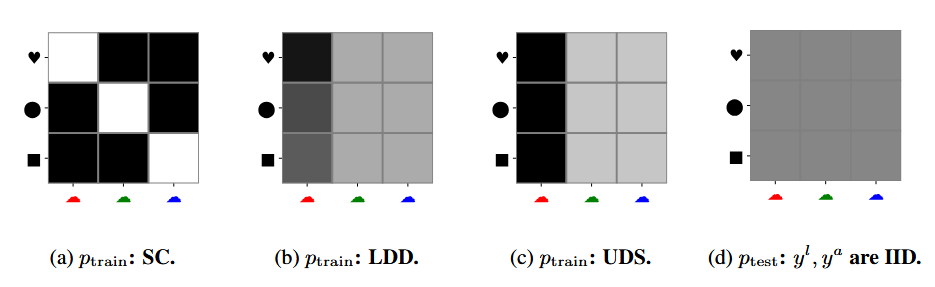
\includegraphics[width=\linewidth]{figure1.png}
  \end{minipage}\hfill
  \caption{Visualization of the joint distribution for the different shifts on the DSPRITES dataset. The lighter the color, the more likely the given example.}
\end{figure}
\end{frame}

% --------------- Additional conditions ----------------
\begin{frame}{Two additional conditions}
The same shifts are studied under two extra ``axes'':

\medskip
\textbf{1. Label noise.}
\begin{itemize}
  \item Observed label $\hat{y}^\ell$ is a noisy version of $y^\ell$ (e.g.\ human rater mistakes).
  \item Vary noise level $p$ and see how methods degrade.
\end{itemize}

\medskip
\textbf{2. Dataset size.}
\begin{itemize}
  \item Fix the shift type, but vary total number of training samples $T$.
  \item Mimics expensive data collection (medical, wildlife).
\end{itemize}
\end{frame}

% ----------------- Benchmark summary -----------------
\begin{frame}{Benchmark: datasets \& methods}
\textbf{Datasets.}
\begin{itemize}
  \item 3 synthetic: DSPRITES, MPI3D, SHAPES3D.
  \item 3 real: SMALLNORB, CAMELYON17 (hospitals), IWILDCAM (camera traps).
  \item For each: choose label $y^\ell$ and nuisance attribute $y^a$ and construct SC, LDD, UDS splits.
\end{itemize}

\medskip
\textbf{Methods (5 families, 19 methods).}
\begin{itemize}
  \item \emph{Architectures}: ResNets, ViT, MLP.
  \item \emph{Heuristic augmentations}: standard ImageNet-style, RandAugment, etc.
  \item \emph{Learned augmentations}: CYCLEGAN-style attribute-conditioned image translation.
  \item \emph{Domain generalization}: IRM, DeepCORAL, DANN, SagNet, etc.
  \item \emph{Pretraining / representations}: ImageNet pretraining, $\beta$-VAE.
\end{itemize}

\end{frame}

\begin{frame}{Benchmark: datasets \& methods}
\begin{figure}[h!]
    \centering
  \begin{minipage}{0.9\textwidth}
    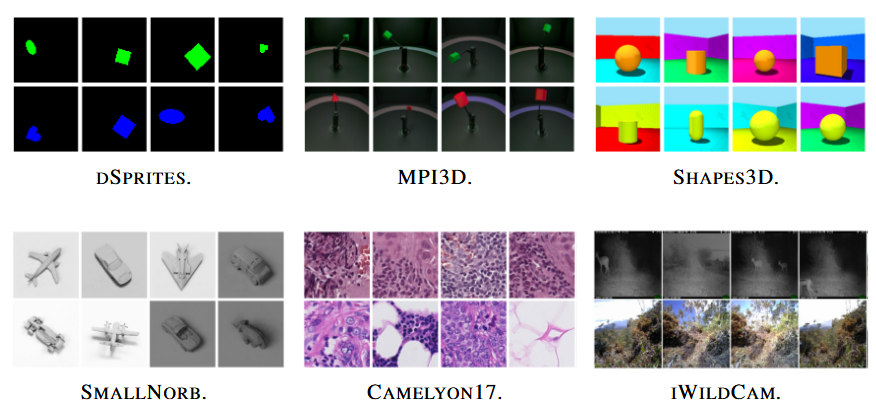
\includegraphics[width=\linewidth]{figure2.png}
  \end{minipage}\hfill
  \caption{Dataset samples. Each row fixes an attribute.}
\end{figure}
\end{frame}

% -------------- Core experimental findings -----------
\begin{frame}{Core experimental findings (1/2)}
\textbf{Across SC, LDD, UDS:}
\begin{itemize}
  \item \textbf{Pretraining} and \textbf{augmentations} (both heuristic and learned) often give the largest gains over plain ERM.
  \item \textbf{Learned augmentation} (CYCLEGAN-style) is especially strong for spurious correlations.
  \item \textbf{Pretraining} is especially strong for low-data and unseen shifts (helps with rare / unseen attribute values).
\end{itemize}

\medskip
\textbf{Domain generalization \& adaptive methods.}
\begin{itemize}
  \item Methods like IRM, DeepCORAL, DANN, SagNet give at best \emph{modest}, inconsistent improvements.
  \item No clear evidence that they systematically beat strong baselines (good architectures + pretraining + augmentations).
\end{itemize}

\end{frame}

\begin{frame}{Core experimental findings (1/2)}
\begin{figure}[h!]
\centering
\begin{minipage}{0.5\textwidth}
  \centering
  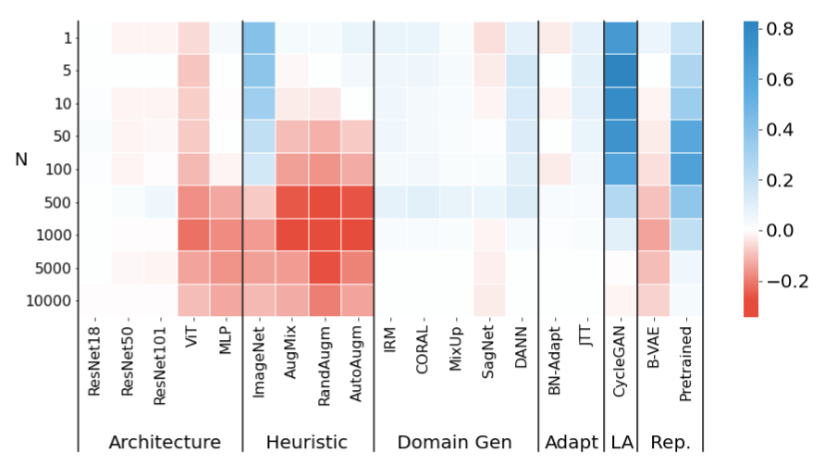
\includegraphics[width=\linewidth]{figure3.png}
  \caption{Spurious Correlation.}
\end{minipage}\hfill
\begin{minipage}{0.5\textwidth}
  \centering
  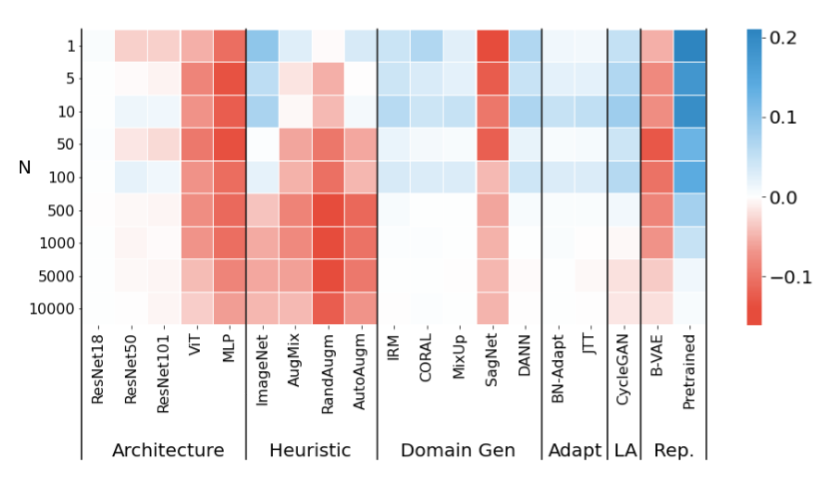
\includegraphics[width=\linewidth]{figure4.png}
  \caption{Low-data drift.}
\end{minipage}
\end{figure}
\end{frame}

\begin{frame}{Core experimental findings (2/2)}
\textbf{Effect of label noise.}
\begin{itemize}
  \item Relative ordering of methods is fairly stable as noise increases.
  \item Pretraining and learned augmentation remain robust; some heuristic aug methods also stable.
\end{itemize}

\medskip
\textbf{Effect of dataset size.}
\begin{itemize}
  \item When $T$ is small, naive augmentations can hurt (too much stochasticity vs.\ signal).
  \item Pretraining and learned augmentations remain useful even with limited data.
\end{itemize}

\medskip
\textbf{No universal winner.}
\begin{itemize}
  \item Best method depends on:
  \begin{itemize}
    \item which shift (SC, LDD, UDS),
    \item which dataset,
    \item and which attribute is treated as nuisance.
  \end{itemize}
\end{itemize}

\end{frame}

\begin{frame}{Core experimental findings (2/2)}
\begin{figure}[h!]
\centering
\begin{minipage}{0.5\textwidth}
  \centering
  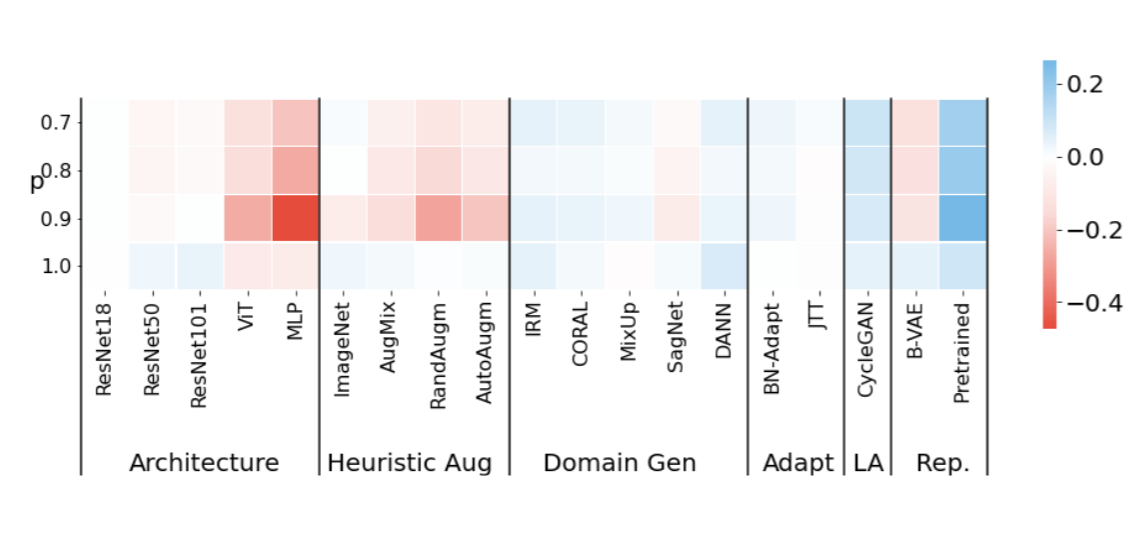
\includegraphics[width=\linewidth]{figure5.png}
  \caption{Noisy labels.}
\end{minipage}\hfill
\begin{minipage}{0.5\textwidth}
  \centering
  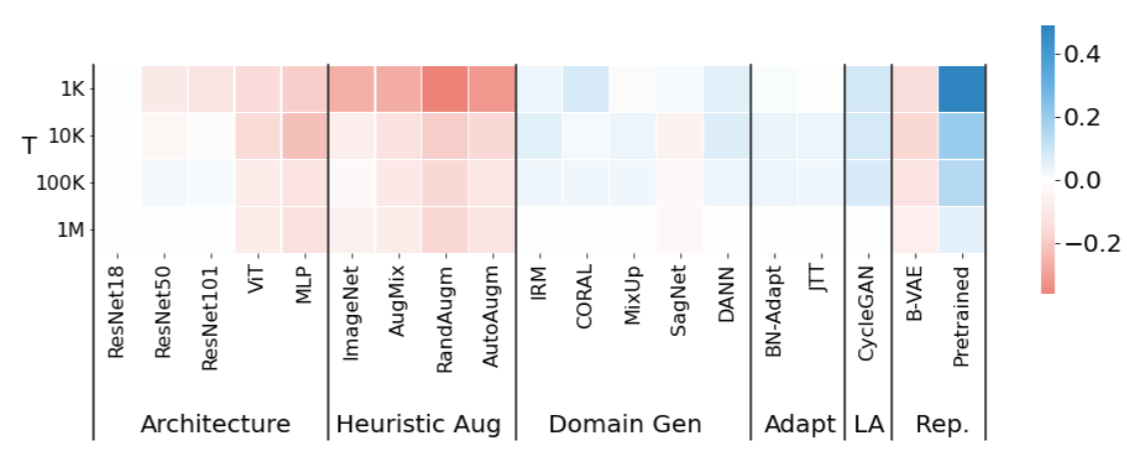
\includegraphics[width=\linewidth]{figure6.png}
  \caption{Fixed data.}
\end{minipage}
\end{figure}
\begin{figure}[h!]
    \centering
  \begin{minipage}{0.6\textwidth}
    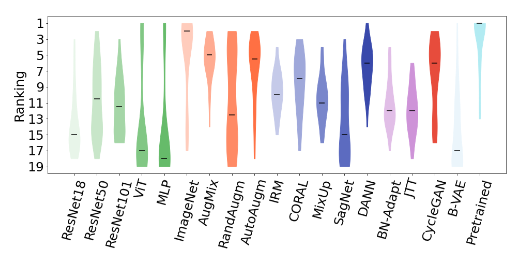
\includegraphics[width=\linewidth]{figure7.png}
  \end{minipage}\hfill
  \caption{Unseen data shift.}
\end{figure}
\end{frame}

% ------------------- Practical takeaways -------------
\begin{frame}{Practical takeaways}
\textbf{1. Start with simple, strong baselines.}
\begin{itemize}
  \item Good architectures + pretraining + well-chosen augmentations.
  \item These often outperform more complex domain-generalization tricks.
\end{itemize}

\medskip
\textbf{2. Match augmentations to expected shifts.}
\begin{itemize}
  \item If you know relevant nuisance factors (color, style, lighting), encode them in augmentation.
  \item When heuristic aug is not enough, learn attribute-conditioned transformations.
\end{itemize}

\end{frame}

% ---------------------- Conclusion -------------------
\begin{frame}{Conclusion}
\begin{itemize}
  \item The paper proposes a \textbf{framework} that views distribution shifts as changes in attribute marginals $p(y^1,\dots,y^K)$ with shared generator $p(\mathbf{x}\mid y^1,\dots,y^K)$.
  \item Within this framework, it defines three core shifts (SC, LDD, UDS) and two conditions (label noise, dataset size), and builds a benchmark across 6 datasets and 19 methods.
  \item Large-scale experiments ($\sim 85$K models) show:
  \begin{itemize}
    \item real progress over ERM, mainly via pretraining and (learned or heuristic) augmentations;
    \item but \textbf{no single method} dominates across all shifts and datasets;
  \end{itemize}
  \item The framework is extensible and can be used to test new methods and more complex shifts.
\end{itemize}
\end{frame}

\end{document}
